\documentclass{article}
\usepackage[pages=some]{background}
\usepackage{eso-pic}
\usepackage{transparent}
\usepackage[utf8]{inputenc}
\usepackage[russian]{babel}
\usepackage{soul}


\title{Deadmind Manual}
\date{Version 0.0.1}

\backgroundsetup{
scale=1,
opacity=0.8,
angle=0,
contents={%
  
\includegraphics[width=\paperwidth,height=\paperheight]{paper.png}
  }%
}
\begin{document}


\BgThispage

\maketitle

\section* {Introduction}
What follows is the operators manual for bomb defusal containing all the knowledge we've learned fighting terror in our great country. We'd like to remind the operator that sharing this manual is grounds for capital treason. Under \textbf{NO} circumstances shall you render any part of the material visible to a third-party or we will prosecute you fully to the extent that the law allows us.

Thank you \& слава россии!
\thispagestyle{empty}
\newpage
\BgThispage
\thispagestyle{empty}
\AddToShipoutPicture*{
    \put(0,50){
        \parbox[b][\paperheight]{\paperwidth}{%
            \vfill
            \centering
            {
                \transparent{0.92}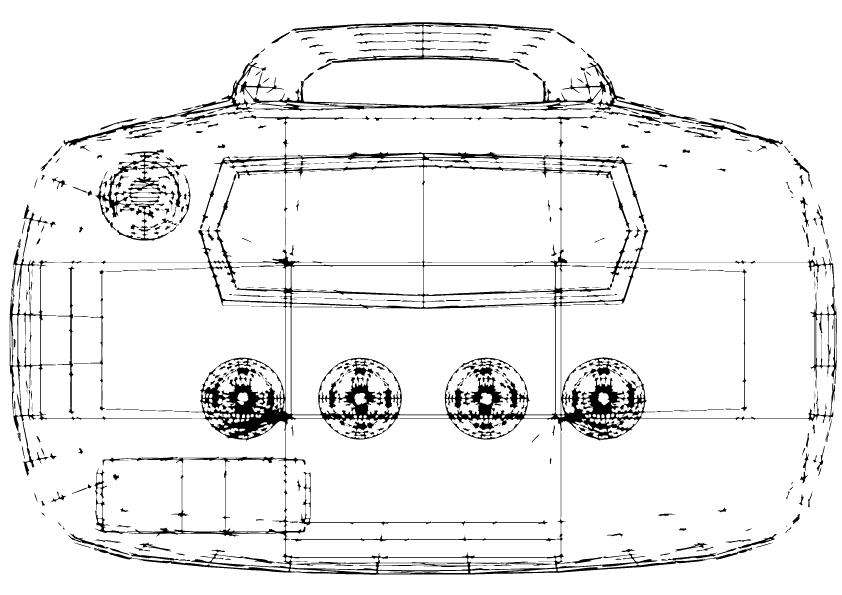
\includegraphics[width=280pt,height=180pt]{b.png}
            }%
            \vfill
        }
    }
}
\section* {Simon Says}

Simon Says is the classic game where the field agents get the information, and they repeat it to you the operator. With a fun twist, get it wrong and \st{you'll regret it}.\\

The field agents will phone back to base with a flashing color and a word, you can use these to relay back information to deactivate the device



\begin{center}
\begin{tabular}{ |p{3cm}||p{2cm}|p{2cm}|p{2cm}|p{2cm}| }
 \hline
 \multicolumn{5}{|c|}{Defuser} \\
 \hline
 Flashing Color -- Word& Red & Green & Blue & Yellow\\
 \hline
 LEED0   & Blue    &Yellow&   Yellow & Red\\
 \hline
 LEAD0   & Green    &Blue&   Red & Yellow\\
 \hline
 YOURE   & Green    &Blue&   Red & Yellow\\
 \hline
 YOURS   & Red    &Blue&   Yellow & Red\\
 \hline
\end{tabular}
\end{center}

\newpage
\BgThispage
\thispagestyle{empty}
\AddToShipoutPicture*{
    \put(0,50){
        \parbox[b][\paperheight]{\paperwidth}{%
            \vfill
            \centering
            {
                \transparent{0.92}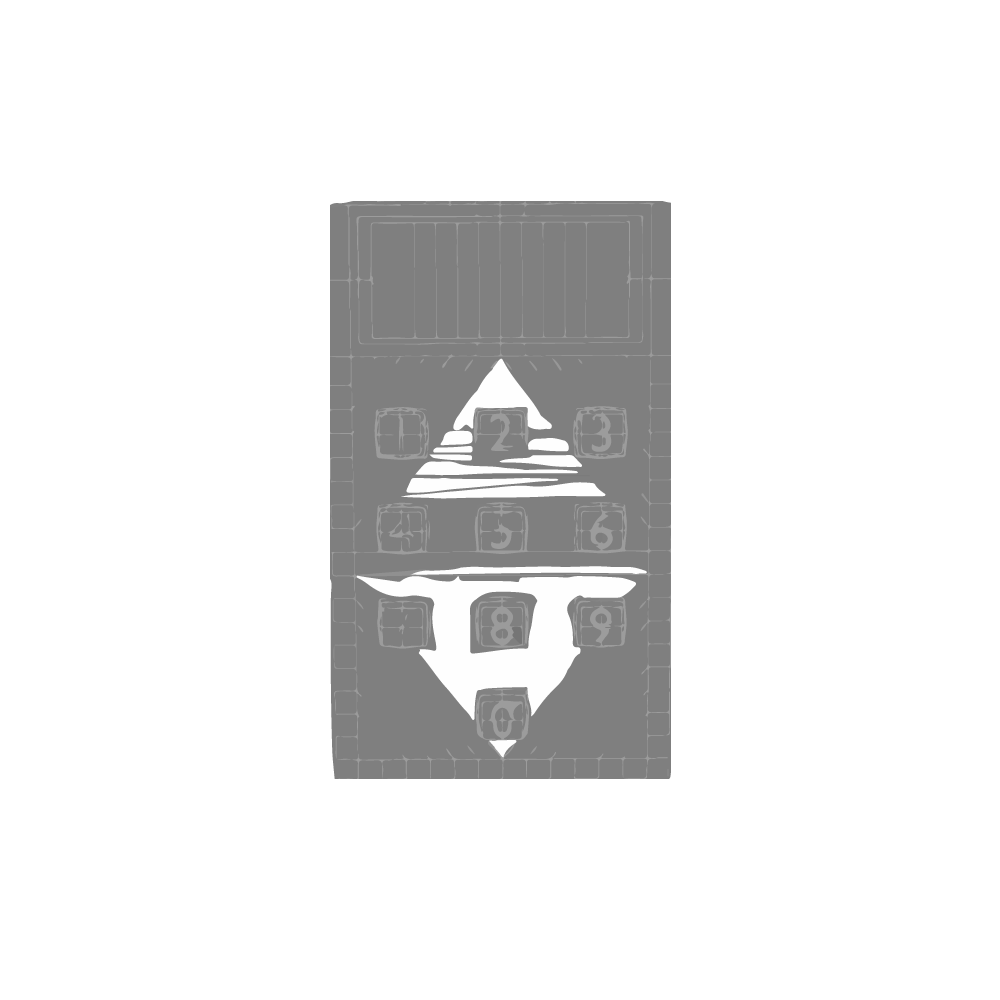
\includegraphics[width=240pt,height=250pt]{keypad.png}
            }%
            \vfill
        }
    }
}

\section* {Symbols}
In certain parts of the deadmind facility we have some \textit{interesting} experiments going on in there, SO that's why we gave the guys down in R\&D a few million to solve the problem, and here's their solution, The deadmind cipher!\\ It's not something for mortal men, really. They made it so that anyone who's not authorized personnel, upon learning about it will have their minds destroyed, forever. Good thing we have you, our trusty certified operator, and if you're not certified I reckon you should stop reading right about here.\\\\
Field agents may encounter a numberpad device that shows a symbol, and they will have to try their best to describe it back to you over the line. It's your job using their description to deduce what numbers they should be pressing on the keypad.
\begin{center}
\begin{tabular}{ |p{2cm}||p{3.5cm}| }
 \hline
 \multicolumn{2}{|c|}{The deadmind cipher} \\
 \hline
 $<$& 0\\
 \hline
 $>$& 1\\
 \hline
 $+$   & 2\\
 \hline
 \$   & 3\\
 \hline
 /   & 4\\
 \hline
 =   & 5\\
 \hline
 \%   & 6\\
 \hline
 *   & 7\\
 \hline
 ?   & 8\\
 \hline
 -   & 9\\
 \hline
\end{tabular}
\end{center}

\newpage
\BgThispage
\thispagestyle{empty}
\section*{Art}
Ah art, the finest humanity has to offer, and we've also been doing some experiments with it at the deadmind facility. But in order to preserve our oh so precious art, we've created decoys and placed them all over the facility to trick the robbers into stealing a fake piece of art, rather than a real one.\\
So where does that leave you operator? You need to help the field agents identify the real piece of art on display. The easiest way to do this is to verify that the painting belong to the correct aristocrat.\\

Here's a simplified version of the facilities manifest:

\subsection*{Pierre Boulanger}
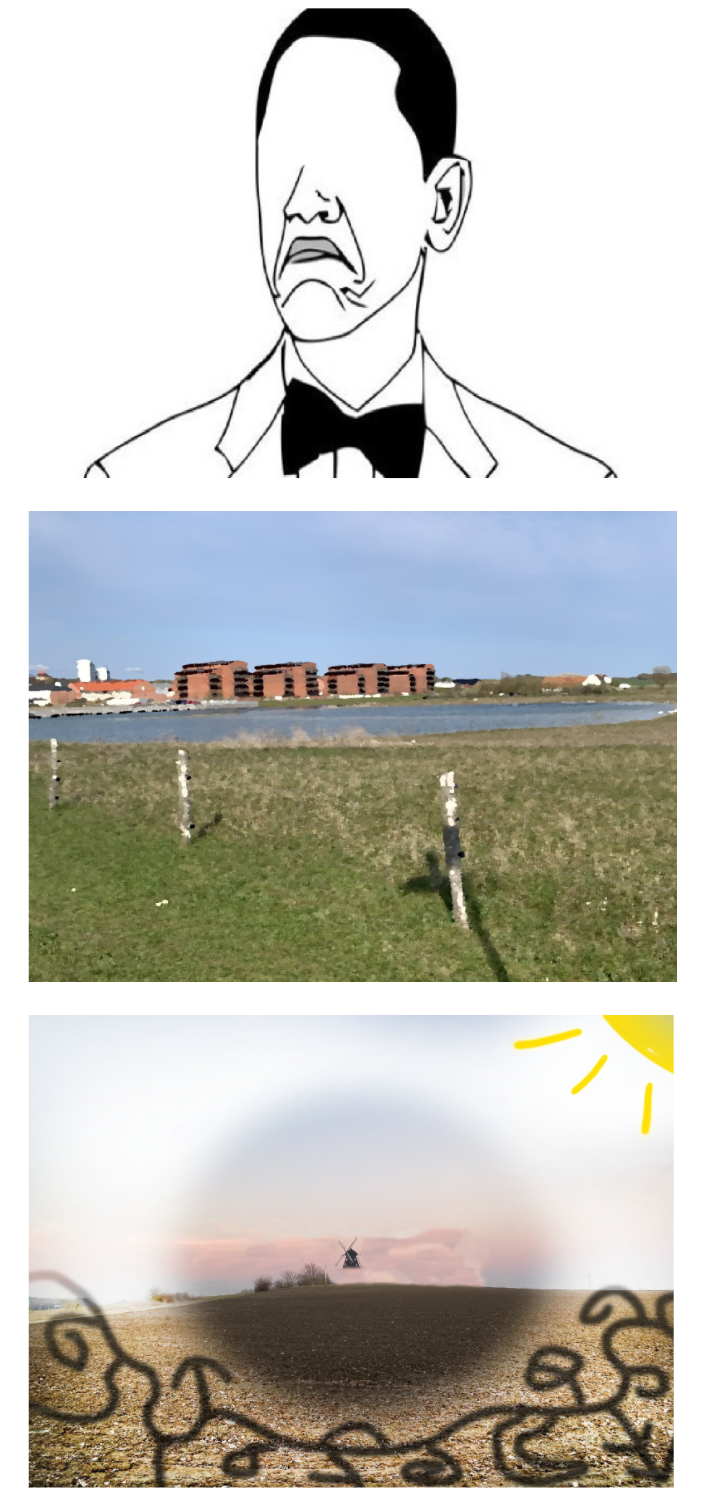
\includegraphics[width=8cm,height=13cm]{Pierre_Boulanger.png}
\newpage
\BgThispage
\thispagestyle{empty}
\subsection*{Jean-Auguste Bonaparte}
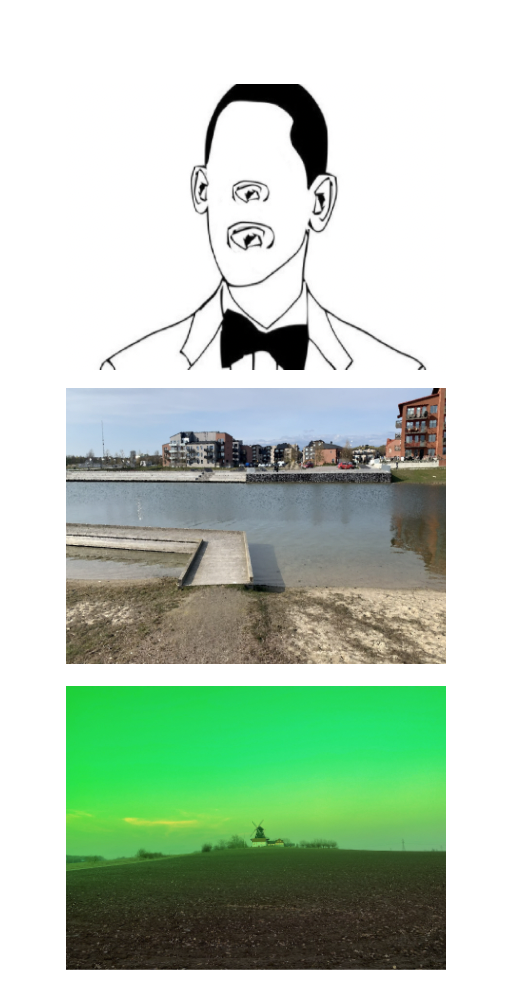
\includegraphics[width=10cm,height=13cm]{Jean_Auguste_Bonaparte.png}
\newpage
\BgThispage
\thispagestyle{empty}
\subsection*{Francois Lacroix}
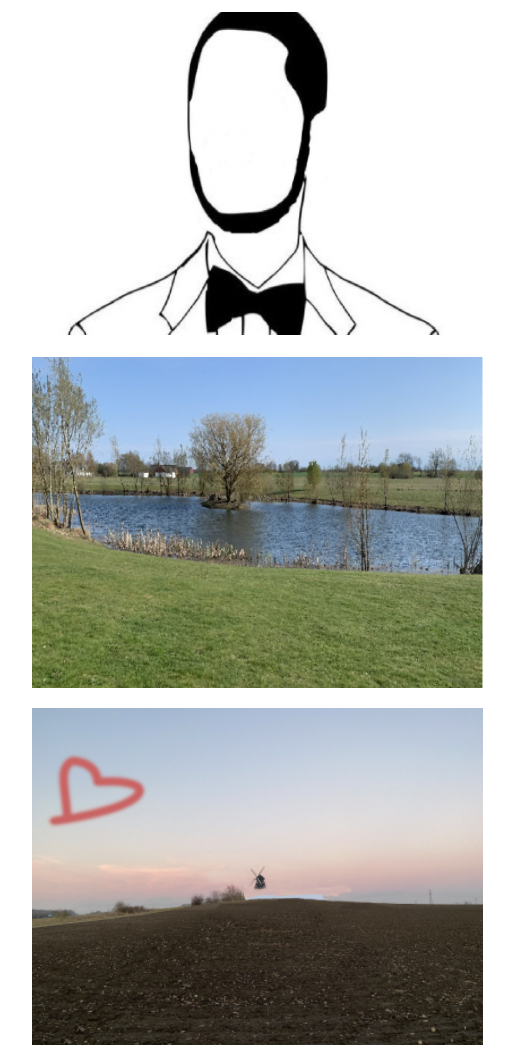
\includegraphics[width=9cm,height=13cm]{Francois_Lacroix.png}

\subsection*{A warning...}
As you can observe a lot of the images are similar, as always communication is key, and communicating the more smaller details is key to complete this objective.

\end{document}

